\documentclass[a4paper,landscape]{article}
\usepackage[margin=1.0cm]{geometry}
\usepackage{tikz}
\usetikzlibrary{positioning, arrows.meta, shapes, shapes.geometric, shapes.misc, fit, backgrounds, calc}
\usepackage{xcolor}

\definecolor{procblue}{RGB}{25,75,150}
\definecolor{procfill}{RGB}{210,228,255}
\definecolor{stgreen}{RGB}{0,110,60}
\definecolor{stfill}{RGB}{210,245,225}
\definecolor{extbrn}{RGB}{135,65,0}
\definecolor{extfillb}{RGB}{255,240,210}
\definecolor{arrgray}{RGB}{80,100,130}

\tikzset{
  PR/.style={draw=procblue,fill=procfill,thick,rounded rectangle,minimum width=2.8cm,minimum height=1.0cm,font=\scriptsize\bfseries\sffamily\color{procblue},align=center,inner sep=3pt},
  DS/.style={draw=stgreen,fill=stfill,thick,rectangle,minimum width=2.6cm,minimum height=0.75cm,font=\scriptsize\sffamily\color{stgreen},align=center,inner sep=2pt},
  EX/.style={draw=extbrn,fill=extfillb,thick,rectangle,minimum width=2.4cm,minimum height=0.8cm,font=\scriptsize\bfseries\sffamily\color{extbrn},align=center,rounded corners=2pt,inner sep=2pt},
  FL/.style={->,>=Latex,thick,arrgray},
  lb/.style={font=\tiny\sffamily,fill=white,inner sep=0.8pt,midway},
}

\begin{document}
\pagestyle{empty}

\begin{center}
  {\Large\bfseries\sffamily\color{procblue} Data Flow Diagram (Level 1) --- Metamorphic Circuit Breaker Framework}\\[3pt]
  {\small\sffamily\color{gray} Metamorphic Circuit Breaker: A Runtime Reliability Layer for Detecting Transform-Brittleness in Deployed Vision Models}
\end{center}
\vspace{4pt}

\begin{center}
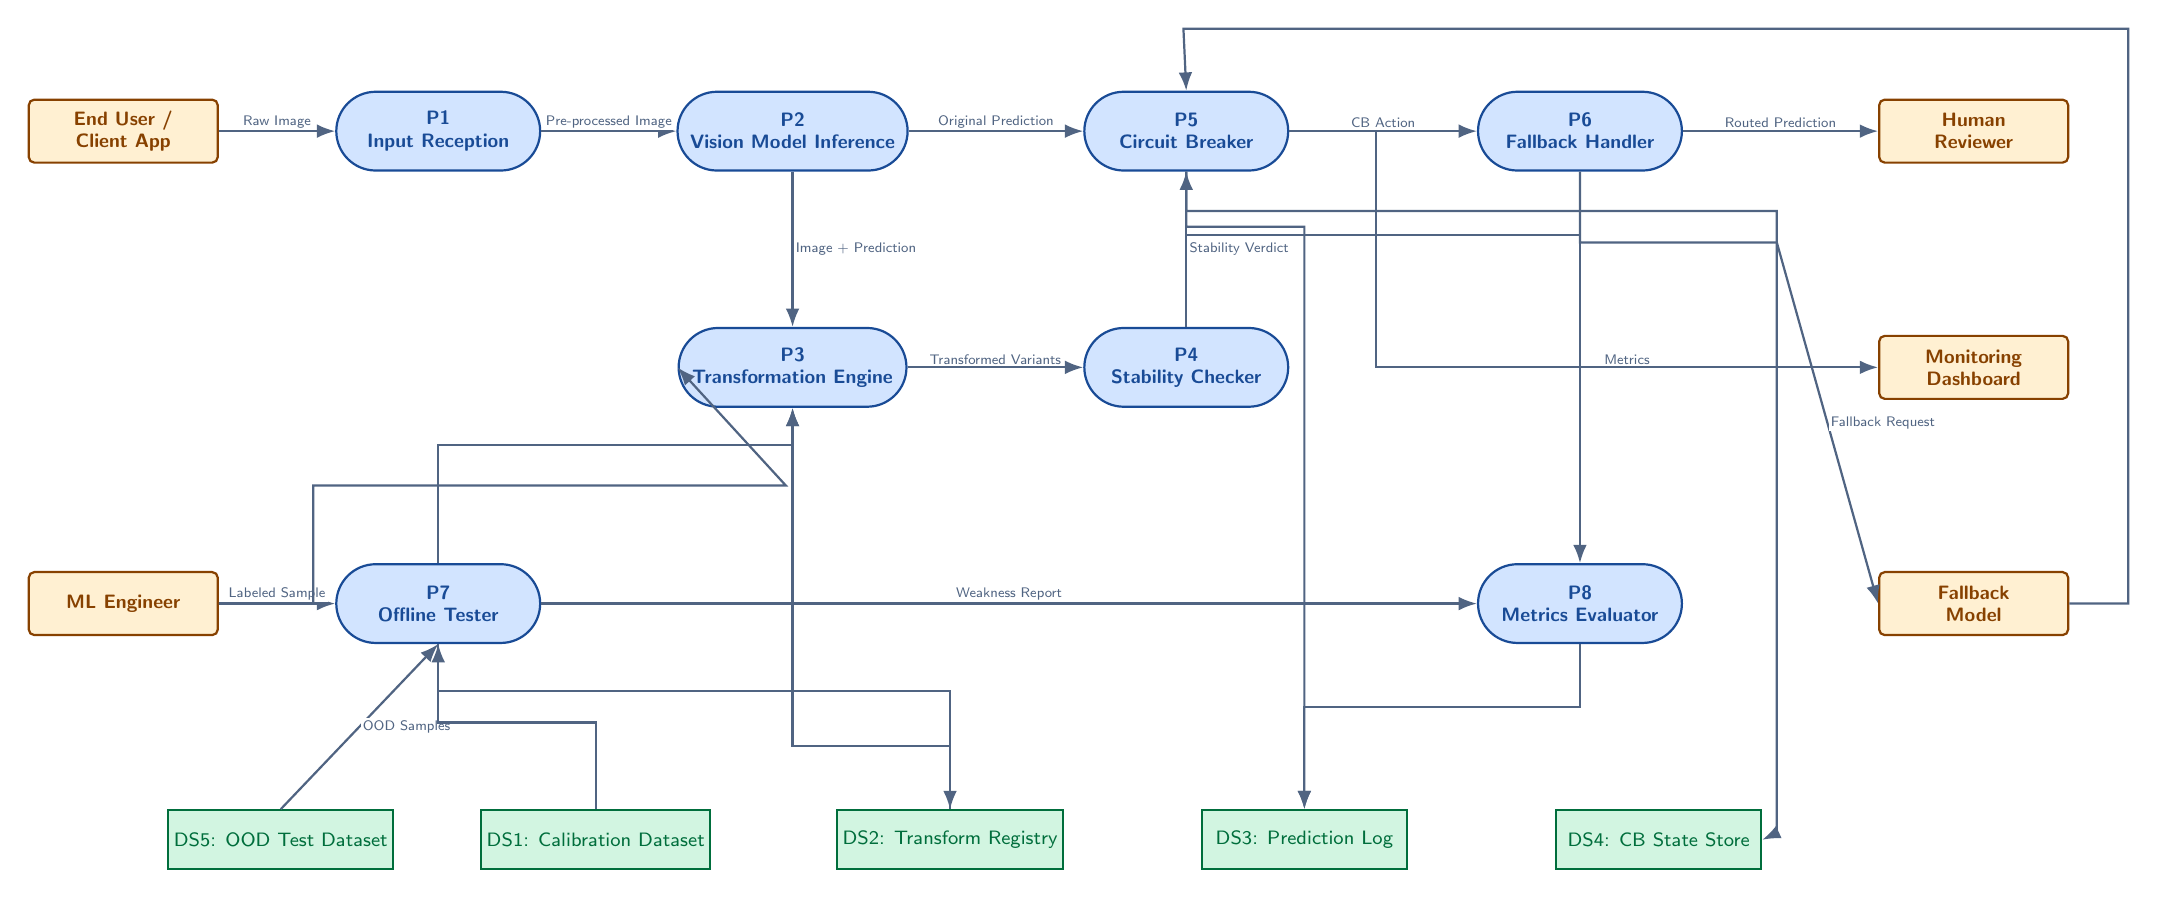
\begin{tikzpicture}[font=\scriptsize\sffamily]

% External entities
\node[EX](user)    at ( 0.0, 4.5){End User /\\Client App};
\node[EX](human)   at (23.5, 4.5){Human\\Reviewer};
\node[EX](monitor) at (23.5, 1.5){Monitoring\\Dashboard};
\node[EX](fbmodel) at (23.5,-1.5){Fallback\\Model};
\node[EX](mleng)   at ( 0.0,-1.5){ML Engineer};

% Processes
\node[PR](p1) at ( 4.0, 4.5){P1\\Input Reception};
\node[PR](p2) at ( 8.5, 4.5){P2\\Vision Model Inference};
\node[PR](p5) at (13.5, 4.5){P5\\Circuit Breaker};
\node[PR](p6) at (18.5, 4.5){P6\\Fallback Handler};
\node[PR](p3) at ( 8.5, 1.5){P3\\Transformation Engine};
\node[PR](p4) at (13.5, 1.5){P4\\Stability Checker};
\node[PR](p7) at ( 4.0,-1.5){P7\\Offline Tester};
\node[PR](p8) at (18.5,-1.5){P8\\Metrics Evaluator};

% Data stores (y=-4.5)
\node[DS](ds5) at ( 2.0,-4.5){DS5: OOD Test Dataset};
\node[DS](ds1) at ( 6.0,-4.5){DS1: Calibration Dataset};
\node[DS](ds2) at (10.5,-4.5){DS2: Transform Registry};
\node[DS](ds3) at (15.0,-4.5){DS3: Prediction Log};
\node[DS](ds4) at (19.5,-4.5){DS4: CB State Store};

% Top row flows
\draw[FL](user.east)--node[lb,above]{Raw Image}(p1.west);
\draw[FL](p1.east)--node[lb,above]{Pre-processed Image}(p2.west);
\draw[FL](p2.east)--node[lb,above]{Original Prediction}(p5.west);
\draw[FL](p5.east)--node[lb,above]{CB Action}(p6.west);
\draw[FL](p6.east)--node[lb,above]{Routed Prediction}(human.west);

% P2 -> P3 -> P4 -> P5
\draw[FL](p2.south)--node[lb,right]{Image + Prediction}(p3.north);
\draw[FL](p3.east)--node[lb,above]{Transformed Variants}(p4.west);
\draw[FL](p4.north)--node[lb,right]{Stability Verdict}(p5.south);

% P5 -> Monitor (routed via x=16.0 gap between p5 and p6)
\draw[FL](p5.east)--++(1.1,0)--++(0,-3.0)--node[lb,above]{Metrics}(monitor.west);

% P6 -> FbModel
\draw[FL](p6.south)--++(0,-0.9)--++(2.5,0)--node[lb,right]{Fallback Request}(fbmodel.west);

% FbModel -> P5 (routed around far right x=25.5 and above top row y=5.8)
\draw[FL](fbmodel.east)--++(0.75,0)--++(0,7.3)--++(-12.0,0)--(p5.north);

% ML Eng -> P7
\draw[FL](mleng.east)--node[lb,above]{Labeled Sample}(p7.west);

% ML Eng -> P3 (routed via y=0.0)
\draw[FL](mleng.east)--++(1.2,0)--++(0,1.5)--++(6.0,0)--(p3.west);

% P7 -> P3
\draw[FL](p7.north)--++(0,1.5)--++(4.5,0)--(p3.south);

% P7 -> P8
\draw[FL](p7.east)--node[lb,above]{Weakness Report}(p8.west);

% P5 -> P8
\draw[FL](p5.south)--++(0,-0.8)--++(5.0,0)--(p8.north);

% Data store flows
\draw[FL](ds5.north)--node[lb,right]{OOD Samples}(p7.south);
\draw[FL](ds1.north)--++(0,1.1)--++(-2.0,0)--(p7.south);

\draw[FL](p7.south)--++(0,-0.6)--++(6.5,0)--(ds2.north);
\draw[FL](ds2.north)--++(0,0.8)--++(-2.0,0)--(p3.south);

\draw[FL](p5.south)--++(0,-0.7)--++(1.5,0)--(ds3.north);
% P5 -> DS4 (routed via x=21.0 corridor, right of P8)
\draw[FL](p5.south)--++(0,-0.5)--++(7.5,0)--++(0,-7.9)--(ds4.east);

\draw[FL](p8.south)--++(0,-0.8)--++(-3.5,0)--(ds3.north);

\end{tikzpicture}
\end{center}

\end{document}
